\documentclass[11pt, a4paper]{jarticle}
% \usepackage{../style/new_coe}
%\usepackage{../style/coe}
\usepackage[dvipdfmx]{graphicx}
\usepackage{wrapfig}
\usepackage{bm}
\usepackage{amsmath, amssymb}
\usepackage{type1cm}
\usepackage{docmute}
\renewcommand{\figurename}{Fig.}
\renewcommand{\tablename}{Table }
\usepackage{caption, subcaption}
\usepackage{comment}

\topmargin=-.4mm
\oddsidemargin=-0.4mm \evensidemargin=\oddsidemargin
\setlength{\textwidth}{160mm}
\usepackage{algorithmic}
\usepackage{algorithm}

% TITLE of the article
\title{タイトル}

% AUTHOR name
\author{名前}

%----------------------------------------------------------------------

\begin{document}
\maketitle

\section{セクション名} %緒言
	参考文献の付け方\cite{キー名}


\section{セクション名} %第2章は理論,手法の説明
	Figureの書き方

	\begin{figure}[htbp]
		\begin{center}
			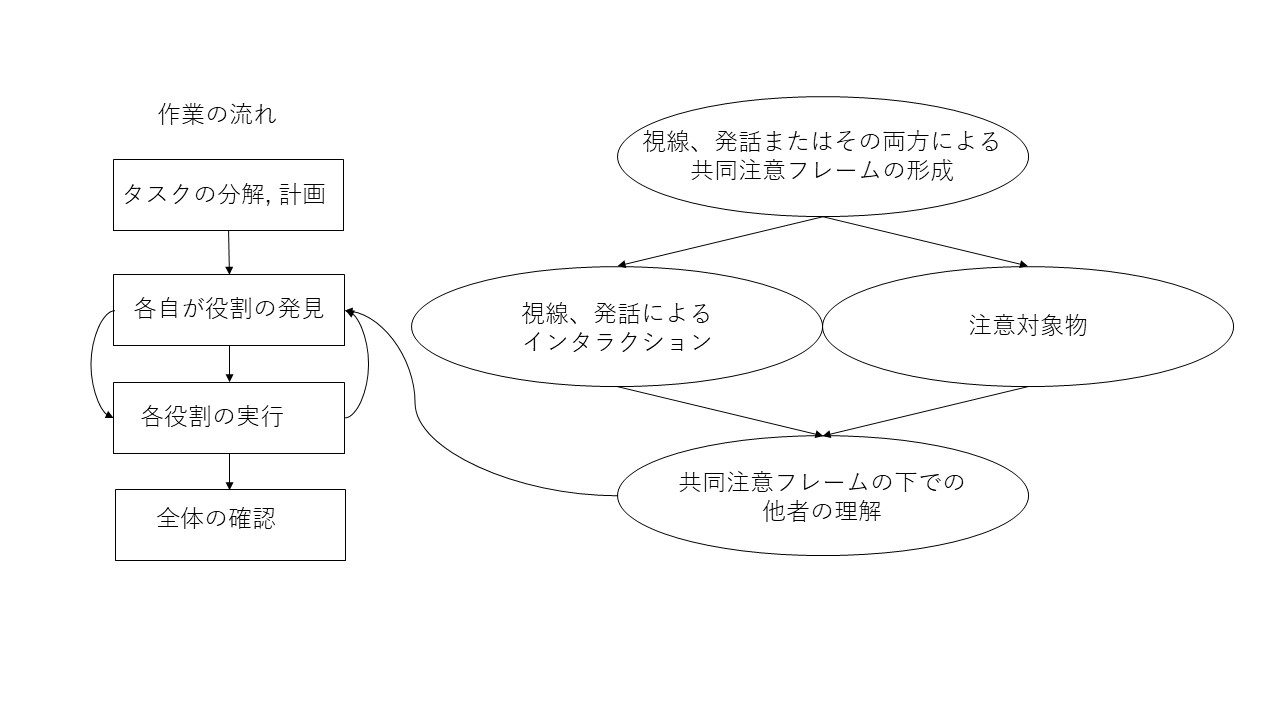
\includegraphics[width = 13.0cm]{../figure/fileName.jpg}
			\caption{キャプション}
		\end{center}
	\end{figure}


\section{セクション名}
	\subsection{サブセクション名}
		箇条書き

		\begin{itemize}
		\item{項目1} \par
		中身1
		\item{項目2} \par
		中身2
		\item{項目3} \par
		中身3
		\end{itemize}


	\subsection{サブセクション名}
		式の書き方($j$, ドルで囲むと文中でも数式扱いになる)

		% _{}で下付き文字, ^{}で上付き文字
		\begin{equation}
			WWL = \frac{\sum_{i=1}^{6}(w_{i}*v_{i})} {\sum_{i=1}^{6}w_{i}}
		\end{equation}

\section{セクション名について} %結言, 今後の展望
	おまけ(\alpha, \beta, \gamma, \Gamma)

\\


\clearpage

\begin{thebibliography}{99}
\bibitem{キー名} 著者名, 論文名, ジャーナル名, バージョン名, ページ名
\end{thebibliography}


\end{document}
